%!TeX root=../wowtop.tex

\ArtChapter[How I Fell In with the Curate]{13head}


\lettrine[lines=4,findent=2pt]{A}{fter} getting this sudden lesson in the power of terrestrial weapons, the Martians retreated to their original position upon Horsell Common; and in their haste, and encumbered with the debris of their smashed companion, they no doubt overlooked many such a stray and negligible victim as myself. Had they left their comrade and pushed on forthwith, there was nothing at that time between them and London but batteries of twelve-pounder guns, and they would certainly have reached the capital in advance of the tidings of their approach; as sudden, dreadful, and destructive their advent would have been as the earthquake that destroyed Lisbon a century ago.

But they were in no hurry. Cylinder followed cylinder on its interplanetary flight; every twenty-four hours brought them reinforcement. And meanwhile the military and naval authorities, now fully alive to the tremendous power of their antagonists, worked with furious energy. Every minute a fresh gun came into position until, before twilight, every copse, every row of suburban villas on the hilly slopes about Kingston and Richmond, masked an expectant black muzzle. And through the charred and desolated area—perhaps twenty square miles altogether—that encircled the Martian encampment on Horsell Common, through charred and ruined villages among the green trees, through the blackened and smoking arcades that had been but a day ago pine spinneys, crawled the devoted scouts with the heliographs that were presently to warn the gunners of the Martian approach. But the Martians now understood our command of artillery and the danger of human proximity, and not a man ventured within a mile of either cylinder, save at the price of his life.

It would seem that these giants spent the earlier part of the afternoon in going to and fro, transferring everything from the second and third cylinders—the second in Addlestone Golf Links and the third at Pyrford—to their original pit on Horsell Common. Over that, above the blackened heather and ruined buildings that stretched far and wide, stood one as sentinel, while the rest abandoned their vast fighting-machines and descended into the pit. They were hard at work there far into the night, and the towering pillar of dense green smoke that rose therefrom could be seen from the hills about Merrow, and even, it is said, from Banstead and Epsom Downs.

And while the Martians behind me were thus preparing for their next sally, and in front of me Humanity gathered for the battle, I made my way with infinite pains and labour from the fire and smoke of burning Weybridge towards London.

I saw an abandoned boat, very small and remote, drifting down-stream; and throwing off the most of my sodden clothes, I went after it, gained it, and so escaped out of that destruction. There were no oars in the boat, but I contrived to paddle, as well as my parboiled hands would allow, down the river towards Halliford and Walton, going very tediously and continually looking behind me, as you may well understand. I followed the river, because I considered that the water gave me my best chance of escape should these giants return.

\begin{wrapfigure}{O}{0.5\textwidth}
\centering
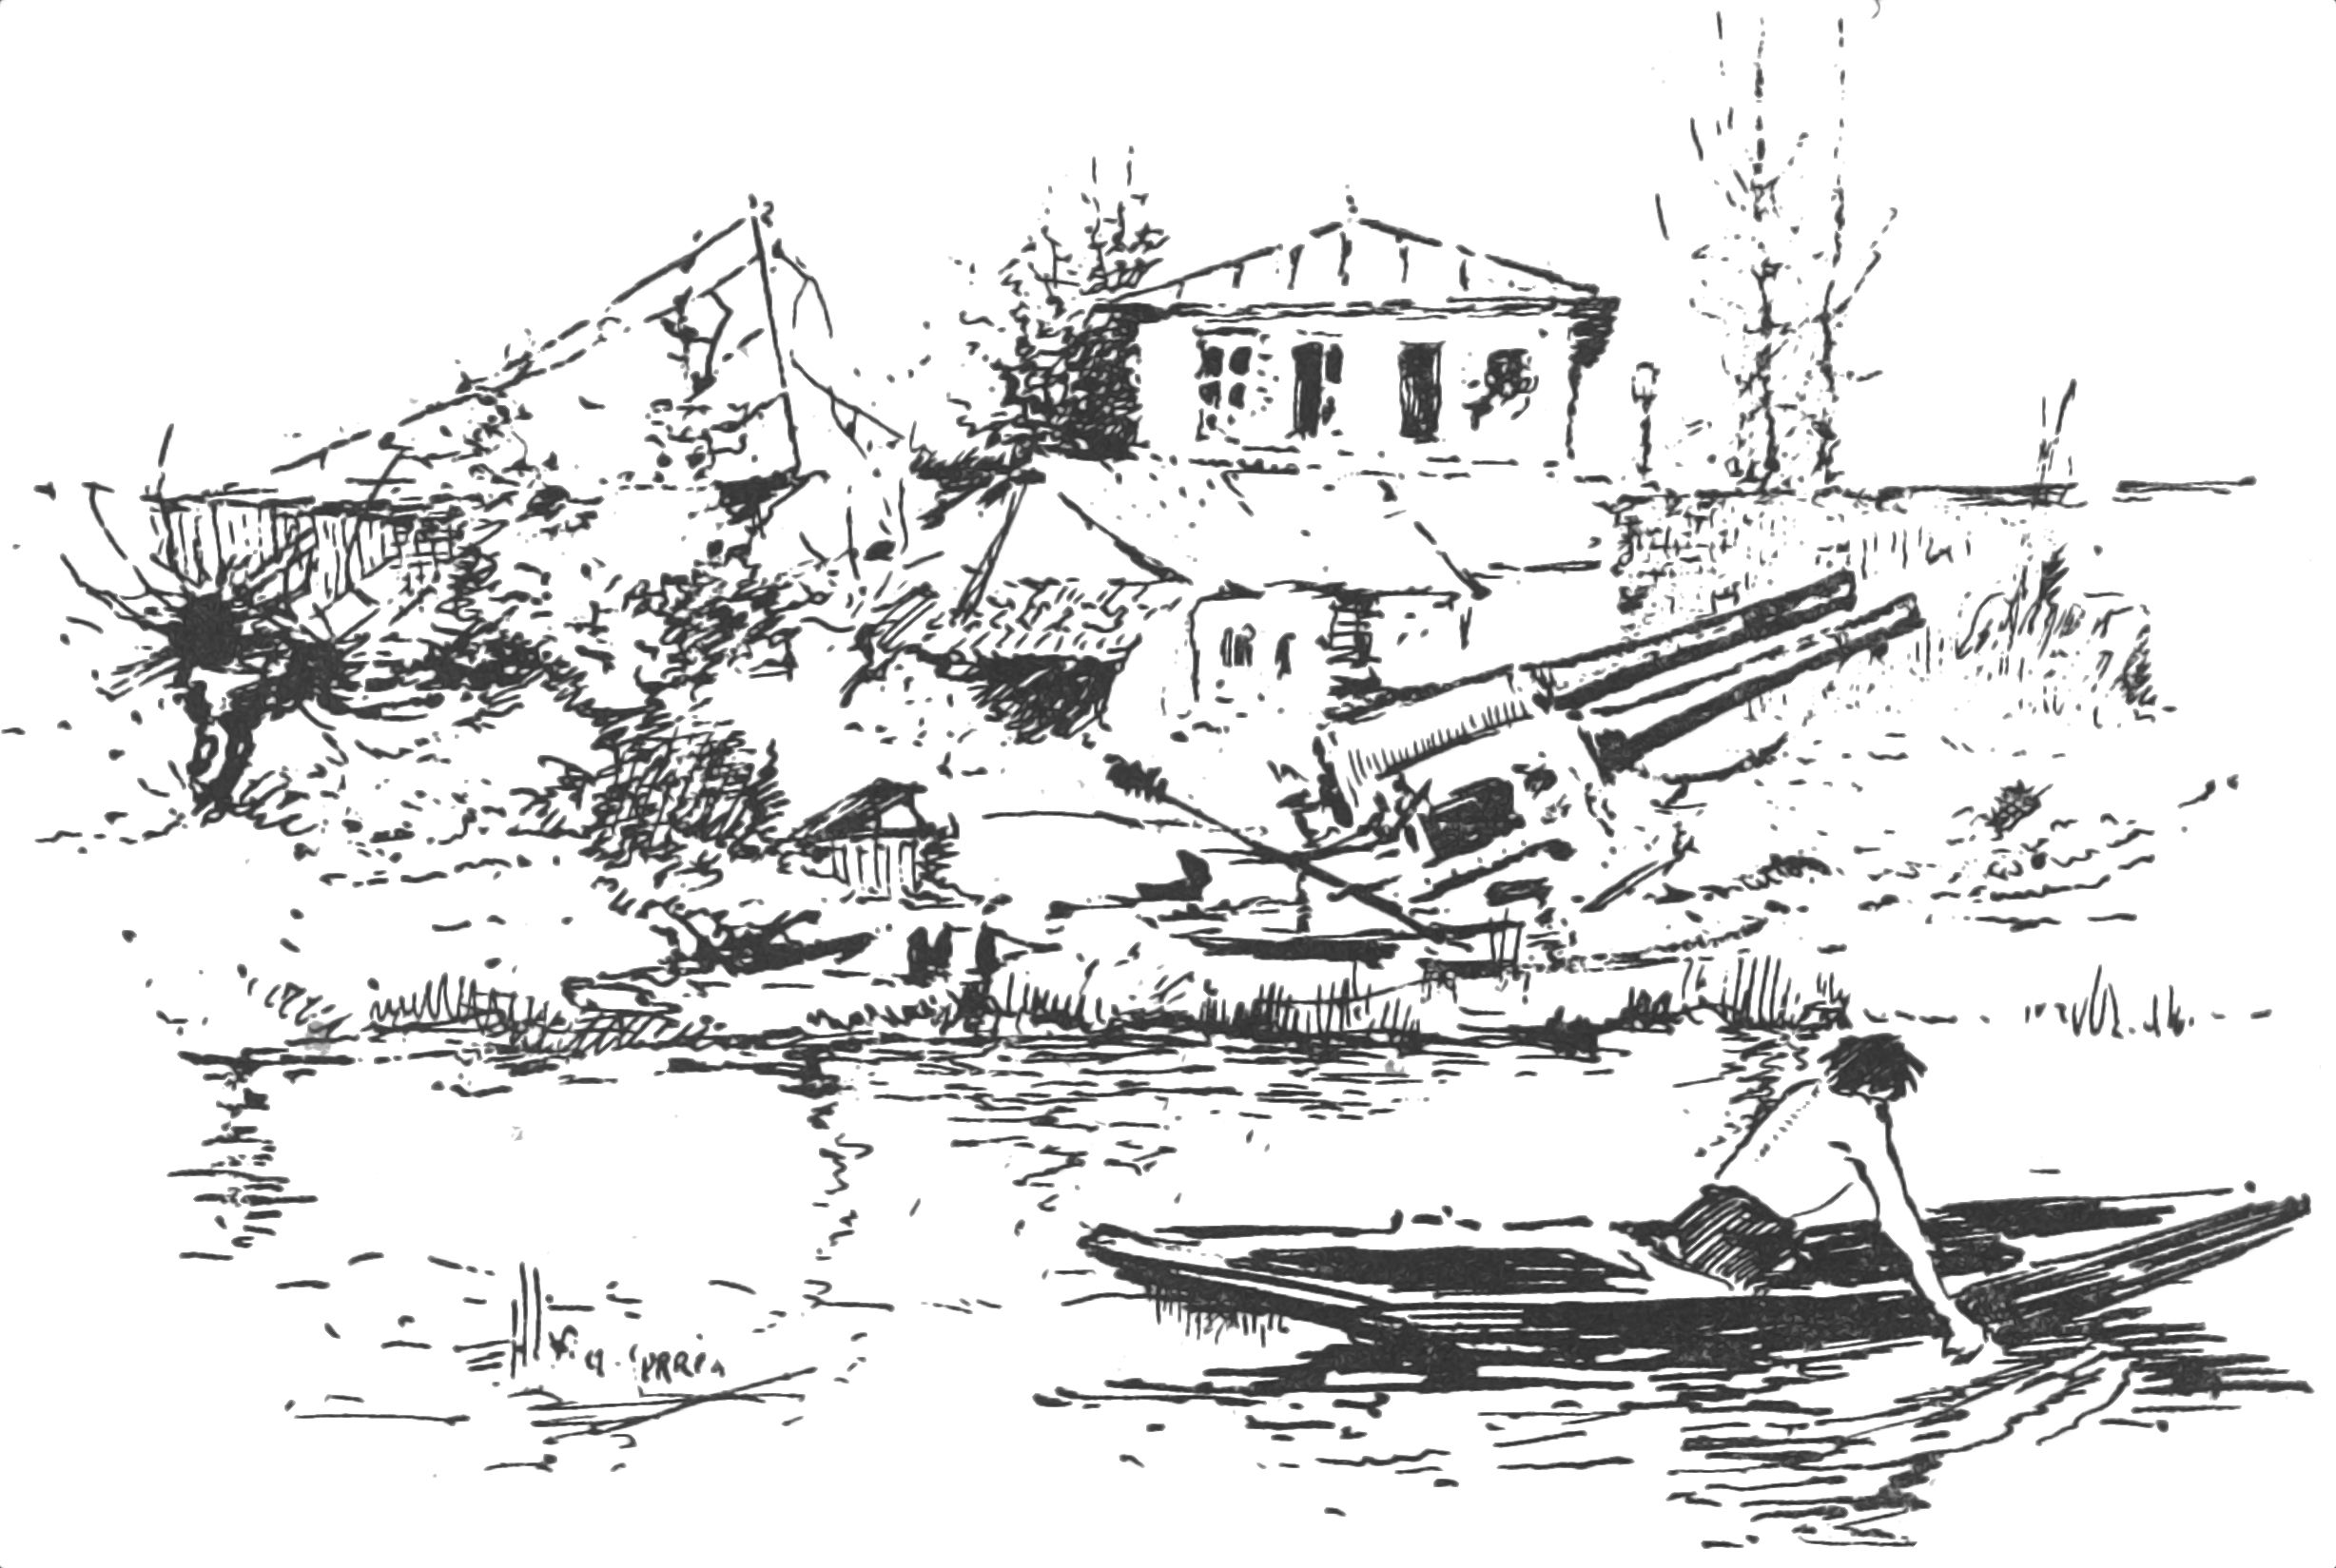
\includegraphics[width=0.5\textwidth]{13boat}
\end{wrapfigure}

The hot water from the Martian's overthrow drifted downstream with me, so that for the best part of a mile I could see little of either bank. Once, however, I made out a string of black figures hurrying across the meadows from the direction of Weybridge. Halliford, it seemed, was deserted, and several of the houses facing the river were on fire. It was strange to see the place quite tranquil, quite desolate under the hot blue sky, with the smoke and little threads of flame going straight up into the heat of the afternoon. Never before had I seen houses burning without the accompaniment of an obstructive crowd. A little farther on the dry reeds up the bank were smoking and glowing, and a line of fire inland was marching steadily across a late field of hay.

For a long time I drifted, so painful and weary was I after the violence I had been through, and so intense the heat upon the water. Then my fears got the better of me again, and I resumed my paddling. The sun scorched my bare back. At last, as the bridge at Walton was coming into sight round the bend, my fever and faintness overcame my fears, and I landed on the Middlesex bank and lay down, deadly sick, amid the long grass. I suppose the time was then about four or five o'clock. I got up presently, walked perhaps half a mile without meeting a soul, and then lay down again in the shadow of a hedge. I seem to remember talking, wanderingly, to myself during that last spurt. I was also very thirsty, and bitterly regretful I had drunk no more water. It is a curious thing that I felt angry with my wife; I cannot account for it, but my impotent desire to reach Leatherhead worried me excessively.

I do not clearly remember the arrival of the curate, so that probably I dozed. I became aware of him as a seated figure in soot-smudged shirt sleeves, and with his upturned, clean-shaven face staring at a faint flickering that danced over the sky. The sky was what is called a mackerel sky—rows and rows of faint down-plumes of cloud, just tinted with the midsummer sunset.

I sat up, and at the rustle of my motion he looked at me quickly.

»Have you any water?« I asked abruptly.

He shook his head.

»You have been asking for water for the last hour,« he said.

For a moment we were silent, taking stock of each other. I dare say he found me a strange enough figure, naked, save for my water-soaked trousers and socks, scalded, and my face and shoulders blackened by the smoke. His face was a fair weakness, his chin retreated, and his hair lay in crisp, almost flaxen curls on his low forehead; his eyes were rather large, pale blue, and blankly staring. He spoke abruptly, looking vacantly away from me.

»What does it mean?« he said. »What do these things mean?«

I stared at him and made no answer.

He extended a thin white hand and spoke in almost a complaining tone.

»Why are these things permitted? What sins have we done? The morning service was over, I was walking through the roads to clear my brain for the afternoon, and then—fire, earthquake, death! As if it were Sodom and Gomorrah! All our work undone, all the work— What are these Martians?«

»What are we?« I answered, clearing my throat.

He gripped his knees and turned to look at me again. For half a minute, perhaps, he stared silently.

»I was walking through the roads to clear my brain,« he said. »And suddenly—fire, earthquake, death!«

He relapsed into silence, with his chin now sunken almost to his knees.

Presently he began waving his hand.

»All the work—all the Sunday schools—What have we done—what has Weybridge done? Everything gone—everything destroyed. The church! We rebuilt it only three years ago. Gone! Swept out of existence! Why?«

Another pause, and he broke out again like one demented.

»The smoke of her burning goeth up for ever and ever!« he shouted.

His eyes flamed, and he pointed a lean finger in the direction of Weybridge.

By this time I was beginning to take his measure. The tremendous tragedy in which he had been involved—it was evident he was a fugitive from Weybridge—had driven him to the very verge of his reason.

»Are we far from Sunbury?« I said, in a matter-of-fact tone.

»What are we to do?« he asked. »Are these creatures everywhere? Has the earth been given over to them?«

»Are we far from Sunbury?«

»Only this morning I officiated at early celebration\longdash«

»Things have changed,« I said, quietly. »You must keep your head. There is still hope.«

»Hope!«

»Yes. Plentiful hope—for all this destruction!«

I began to explain my view of our position. He listened at first, but as I went on the interest dawning in his eyes gave place to their former stare, and his regard wandered from me.

»This must be the beginning of the end,« he said, interrupting me. »The end! The great and terrible day of the Lord! When men shall call upon the mountains and the rocks to fall upon them and hide them—hide them from the face of Him that sitteth upon the throne!«

I began to understand the position. I ceased my laboured reasoning, struggled to my feet, and, standing over him, laid my hand on his shoulder.

»Be a man!« said I. »You are scared out of your wits! What good is religion if it collapses under calamity? Think of what earthquakes and floods, wars and volcanoes, have done before to men! Did you think God had exempted Weybridge? He is not an insurance agent.«

For a time he sat in blank silence.

»But how can we escape?« he asked, suddenly. »They are invulnerable, they are pitiless.«

»Neither the one nor, perhaps, the other,« I answered. »And the mightier they are the more sane and wary should we be. One of them was killed yonder not three hours ago.«

»Killed!« he said, staring about him. »How can God's ministers be killed?«

»I saw it happen.« I proceeded to tell him. »We have chanced to come in for the thick of it,« said I, »and that is all.«

»What is that flicker in the sky?« he asked abruptly.

I told him it was the heliograph signalling—that it was the sign of human help and effort in the sky.

»We are in the midst of it,« I said, »quiet as it is. That flicker in the sky tells of the gathering storm. Yonder, I take it are the Martians, and Londonward, where those hills rise about Richmond and Kingston and the trees give cover, earthworks are being thrown up and guns are being placed. Presently the Martians will be coming this way again.«

And even as I spoke he sprang to his feet and stopped me by a gesture.

»Listen!« he said.

From beyond the low hills across the water came the dull resonance of distant guns and a remote weird crying. Then everything was still. A cockchafer came droning over the hedge and past us. High in the west the crescent moon hung faint and pale above the smoke of Weybridge and Shepperton and the hot, still splendour of the sunset.

»We had better follow this path,« I said, »northward.«

\begin{figure}[b!]
\centering
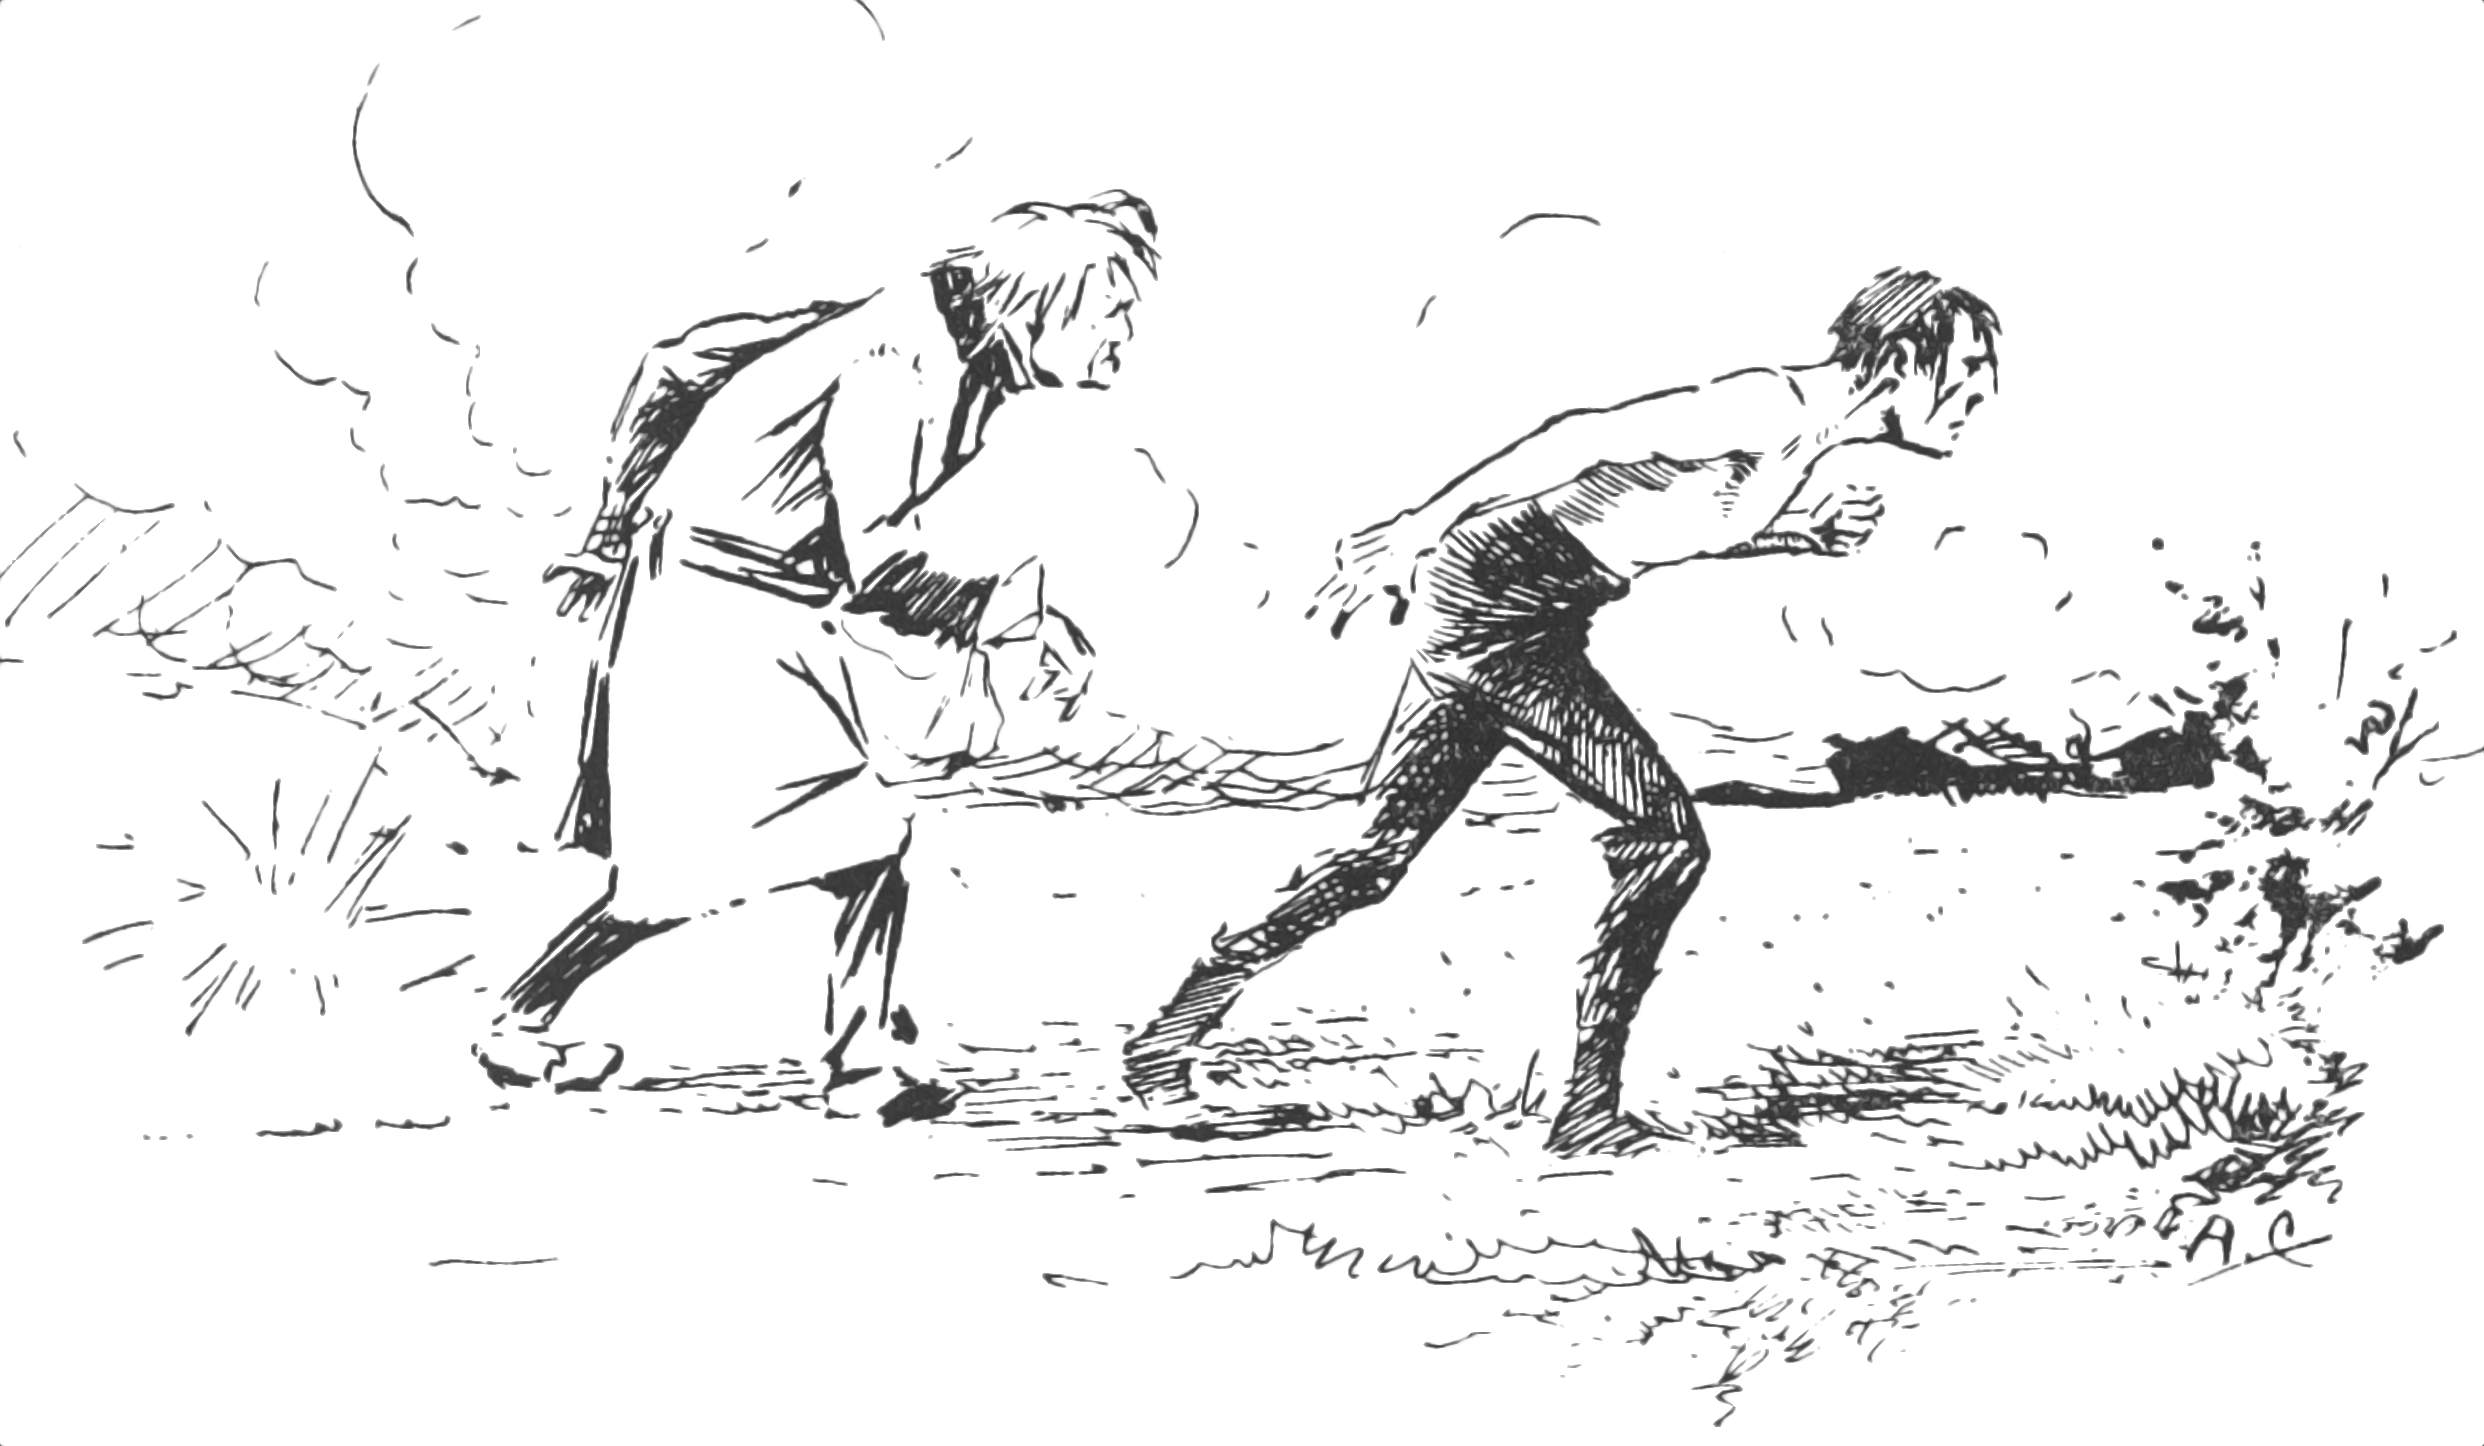
\includegraphics[width=0.7\textwidth]{13tailpiece}
%\captionlistentry{Tailpiece to Chapter \thechapter}
\end{figure}